\chapter{Introduction} \label{ch:intro}

%% =====================================================================================
%%
%%              G E N E R A L  I N T R O D U C T I O N
%%
%% =====================================================================================

%% From Just
A pair of massive stars at the end of their evolution undergo \acp{SN} explosions,
leaving, if stars are sufficiently massive, a pair of compact objects orbiting each other. 
Of particular interest, is a pair of \acp{NS}, compact, but heavy objects sustained 
against gravitational collapse by the neutron degeneracy pressure. 
The theory of \ac{GR} predicts that the orbit of the system shrinks, as \acp{NS} loose energy 
and angular momentum to \acp{GW}. The stars inspiral until they merge at the last orbit. 
%ejecting a small fraction of matter into the Universe, leaving a \pmerg{} remnant.


The high compactness of \acp{NS} leads to an energetic, explosive merger, where a small 
fraction of \ac{NS} matter is ejected from the system at mildly relativistic 
velocities. 
Additionally, the massive \pmerg{} remnant and sorrounding it gravitationally bound 
matter are subjected to complex dynamical interactions, weak processes and magnetically induced 
turbulence, that might be cause matter outflows after merger. This makes \ac{BNS} mergers 
strong contributors to the cosmic chemical evolution. 
The matter ejected at/after mergers, \ie, ejecta, has unique properties, rarely found in other 
astrophysical sites. Specifically, the abundance of free neutrons allow for the so-called 
rapid neutron capture process (\rproc{}), 
The \rproc{} is responsible for the production of the heaviest elements in the 
Universe, lanthanides and actinides. 

%Mergers of \acp{BNS} are at the center of a variety of physical processes in astrophysics.
Wide range of possible types and properties of ejecta lead to a similarly broad 
range in \ac{EM} counterparts to \ac{BNS} mergers. For instance, heavy elements 
produced via \rproc{} \nuc{} eventually decay, powering the quasi-thermal \ac{EM} 
counterpart, \ac{kN}, that can be observed from days to weeks after the merger. 
Additionally, \ac{BNS} mergers are expected to produce 
powerful jets, that can be observed as \acp{SGRB}, whose afterglow lasts for hundreds of days. 
Moreover, expanding into the \ac{ISM} 
medium, mildly relativistic ejecta is expected to generate non-thermal afterglow emission
that can be observed years. 
%Perhaps, two of the most 
%well studied ones are the \ac{kN}, a thermal counterpart powered by the decay of 
%newly synthesized heavy elements in the ejecta, and \acp{SGRB}, generally non-thermal 
%emission from the ultrarelativistic collimated outflow, formed after the merger. 
Together with \ac{GW} emission, these signals allow to study the processes occuring 
at mergers with great details. Studies of \ac{BNS} mergers are crucual for 
investigating the origin of the \ac{SGRB} and cosmic chemical evolution. 
Perhaps most importantly, however, they provide unique constraints on the 
theory of gravity and density of matter at many times the nuclear saturation densities, 
high density part of \ac{NS} \ac{EOS}. 
%Study of these \ac{EM} counterparts in conjuncture with \acp{GW} emission allows to 
%gain unique insigts into the inner workings of the \ac{BNS} merger and previously 
%unobtainable constraints on the theory of gravity, the properties of matter at 
%supranuclear densities, origin of the \ac{SGRB}, cosmic chemical evolution. 



In August 2017, the first \ac{BNS} merger was observed 
as a source of \ac{GW} waves by \ac{LIGO}/Virgo, \GW{}. The unprecedented \ac{EM} 
follow-up campaign, spanning hundreds of observatories across the world lead to 
the identification of the merger \ac{EM} counterparts: \ac{kN}, \AT{} and 
\ac{SGRB}, \GRB{} and compilation of the large amount of data
\citep{TheLIGOScientific:2017qsa,Abbott:2018wiz,GBM:2017lvd}. 
The process, that continues to this day \citep{Hajela:2021faz}.
%
And while \acp{GW} had shed light on the properties of cold matter 
at supernuclear densities, the \ac{NS} \ac{EOS} 
\citep{Hinderer:2009ca,Damour:2012yf,DelPozzo:2013ala}, 
the properties of matter at densities several times that of the 
nuclear matter, as well as the astrophysical implications of the merger 
were largely derived from the \ac{EM} signals 
\citep{Villar:2017wcc,Hajela:2019mjy,Radice:2018ozg,LIGOScientific:2017ync}.

The complexity, non-linearity, non-stationarity and multidimensionality of physical 
processes operating at \ac{BNS} mergers on a wide range of scales of length and time 
implies that self-consistent, quantitative studies are only possible with numerical 
simulations 
\citep{Sekiguchi:2011zd,Wanajo:2014wha,Foucart:2015gaa,Palenzuela:2015dqa,Sekiguchi:2016bjd,Kiuchi:2017zzg,Radice:2017zta,Fujibayashi:2017puw,Radice:2018pdn}.
%
These simulations, performed with \ac{NR} codes that took years, sometimes 
decades to develop and test, are very computationally expensive, rare, and require detailed 
postprocessing and analysis. 
%
Moreover, the self-consistent modeling of the \ac{BNS} merger and its \ac{EM} counterparts 
is still beyond the reach of modern methods. Generally, the short-term (hundred of milliseconds) 
evolution of the merger itself is handled with \ac{NR} codes while the 
\nuc{} and \ac{EM} emission are computed after, in postprocessing. 
%Strengthening the connection between these methods is one of the goals of this thesis. 
%
%In the following sections we sketch the astrophysical background to clarify the 
%context of our study and we conclude the chapter by summarizing the main points of 
%motivation for this thesis and its structural arrangement.

%In this thesis we postprocess a large set of \ac{NR} \ac{BNS} merger simulations, 
%performed with the state-of-the-art \ac{NR} code, \wisky{}, and targeted to the 
%\GW{} (with corresponding binary parameters).
%%
%We focus on the \pmerg{} matter dynamics and properties of ejecta. 
%We asses the nucleosynthetic yields in the ejecta, placing them into astrophysical 
%context. Using the \ac{kN} model, developed by \citet{Perego:2017wtu}, we analyze 
%the \ac{EM} signatures of our \ac{BNS} merger models, comparing them with \AT{}. 
%Additionally, we develop a new code to model non-thermal emission from ejecta 
%expanding into \ac{ISM}, apply it to the outcome of the merger simulations and 
%compare the results with recently observed change in \ac{SGRB} emission. 
%
The main goal of this thesis is to strengthen the link between the ab-inito 
numerical relativity simulations of \ac{BNS} mergers and their 
\ac{EM} signatures, 
and in doing so, provide better constraints on the properties of \GW{} 
and ultimately, \ac{NS} \ac{EOS}.



%Single \acp{NS} are very compact but massive objects, 
%%where compactness $C_{i} = GM_i/R_i^2c^2\propto0.15$ and 
%for description of which the effects of \ac{GR} cannot be neglected. 
%%
%A pair of \acp{NS} orbiting each other slowly loses its 
%angular momentum to \acp{GW}. 
%%The timescale for the radiation reaction, however, 
%%is much longer than the orbital period for most of the inspiral and the 
%%system evolution can be considered adiabatic. 
%%For instance, the inspiral can be considered as a sequence of circular orbits. 
%%However, during last orbits before merger, the finite size (tides) and \ac{HD}
%%effects starts to become important. 
%The inspiral ends at the onset of the Roche lobe overflow, when the binary 
%reaches the mass-shedding limit \citep{Bejger:2004zx}.
%
%%% <<< From Radice Review >>>
%Mergers of \acp{BNS} are at the center of a variety of physical processes 
%in astrophysics.
%The first ever detection of such event by \ac{LIGO}/Virgo, \GW{}, 
%followed up by detections across \ac{EM} spectrum 
%have significantly advanced our understanding 
%of gravity, physics of dense matter, origins of \acp{SGRB} and \rproc{} elements 
%\citep{TheLIGOScientific:2017qsa,Abbott:2018wiz,GBM:2017lvd}. 
%%
%Specifically, while \acp{GW} shed light on the properties of cold matter 
%at supernuclear densities, the \ac{NS} \ac{EOS} 
%\citep{Hinderer:2009ca,Damour:2012yf,DelPozzo:2013ala}, 
%the properties of matter at densities several times that of the 
%nuclear matter, as well as the astrophysical implications of the merger 
%were largely derived from the \ac{EM} signals. 
%
%%Emitted during the inspiral, \acp{GW} delivered a plethora of information about  
%%\ac{NS} \ac{EOS} at supernuclear densities 
%%\citep{Hinderer:2009ca,Damour:2012yf,DelPozzo:2013ala}. 
%%%
%%The properties of matter at densities several times that of the 
%%nuclear matter, however, were not well constrained, as the \pmerg{} \ac{GW} 
%%was not detected. Future observations of the high frequency \pmerg{} signal 
%%will shed more light on these properties 
%%\citep{Sekiguchi:2011mc,Radice:2017lry,Most:2018eaw,Bauswein:2018bma}, 
%%constraining one of the main quantities, the tidal deformability.
%
%The \ac{EM} signal originates from the matter ejected during or after 
%the merger by a variety of physical processes, the so-called, ejecta.
%%
%The conditions within ejecta, are such that the rapid neutron capture (\rproc{}) 
%\nuc{}, responsible for the production of the heaviest elements in the Universe
%such as gold can take place \citep{Cowan:2019pkx}.
%%
%Notably, whether \acp{BNS} mergers are the prime source of this material is still unknown.
%% This was confirmed by \ac{MM} observations of \GW{} \cite{12}. 
%% however, it is unclear whether \ac{BNS} mergers is the dominant source of 
%% \rproc{} elements in the universe, or if other \rproc{} cites are required to 
%% explain the observed abundances in the oldest stars, \ac{UFG} and our solar system. 
%
%
%
%In order to study the dynamical phase of \ac{BNS} mergers and \pmerg{} evolution, 
%sophisticated \ac{NR} simulations are required. Modern, state-of-the-art methods 
%include full \ac{GR}; composition-dependent nuclear \ac{EOS} with finite-temperature 
%effects, \ac{GRMHD} and advanced neutrino transport with varying degree of approximation,
%\citep{Sekiguchi:2011zd,Wanajo:2014wha,Foucart:2015gaa,Palenzuela:2015dqa,Sekiguchi:2016bjd,Kiuchi:2017zzg,Radice:2017zta,Fujibayashi:2017puw}.
%
%%In this thesis we perform \ac{NR} simulations of \ac{BNS} mergers, report on their 
%%qualitative and quantitative picture and its implication for the \ac{EM} signatures.
%%We focus on the nuclear astrophsyics aspect of the mergers, and on the comparison 
%%between theoretical predictions and observations of \GW{}, discussing the 
%%\rproc{} \nuc{}, thermal \ac{EM} transient, and non-thermal \ac{EM} afterglow. 


%% =====================================================================================
%%
%%              T H E O R E T I C A L  P I C 
%%
%% =====================================================================================

\section{Theoretical picture of \ac{BNS} mergers}

In this section we provide a brief summary of the current picture of 
\ac{BNS} mergers, that is largely derived from \ac{NR} simulations.
We also overview their impact on the galactic chemical evolution, and their 
\ac{EM} counterparts. 
%
The section is largely based on the recent reviews from 
different leading groups working on \ac{BNS} merger simulations 
\citep{Radice:2020ddv,Bernuzzi:2020tgt,Shibata:2019wef} 
and their \ac{EM} signatures 
\citep{Kumar:2014upa,Fernandez:2015use,Metzger:2019zeh}.
%to which we refer to for more details and references.
%
For the sake of brevity we allude most of the technical details, 
and we refer the interested reader to the aforementioned  
reviews and references therein.


\subsection{Inspiral}\label{sec:intro:inspiral}

The inspiral phase of the \ac{BNS} system is primarily governed by the emission 
of \acp{GW}. Several approximations exists to describe this phase.
When stars are sufficiently far apart, the \ac{PN} approximation to \ac{GR} 
(the expansion in $\upsilon/c$, with $\upsilon/c\ll 1$, $\upsilon$ 
being the speed of matter) can be used. 
%The dynamics of two stars, that are sufficiently separated to have relatively small 
%angular velocity can be described via the \ac{PN} approximation to \ac{GR} 
%(the expansion in $\upsilon/c$, with $\upsilon/c\ll 1$). 
%In reality, however, \acp{NS} are not point-masses. The finite size (tidal) effects 
%modify the inspiral and, consequently, emitted \acp{GW}. 
Another approximation to the two-body dynamics in \ac{GR} is the \ac{EOB} formalism,
which is a Hamiltonian formalism, applicable to all stages of the binary evolution.
%
The latter has the advantage of taking into account the finite size of \acp{NS}, \ie, 
how the gravitational field of one star affects another. 
These are the so-called tidal effects. 
Their description involves the stars' dimensionless relativistic Love numbers \citep{Damour:2009vw,Binnington:2009bb}, which 
%in the case of quasi-static external field 
if the stars are sufficiently far apart, 
can be computed by considering the stationary perturbations 
of a spherical relativistic star, \ie, solving the stellar structure, 
\ac{TOV}, equations in full \ac{GR}.
% taking into account the strong dependency of the 
%tidal coefficients on the star compactness, defined as $C_{i} = GM_i/R_i^2c^2$. 
These, Love numbers carry the imprint of an \ac{EOS} on the \ac{BNS} dynamics.
%
The inclusion of tidal effects manifests as a faster inspiral and merger at higher 
frequency of \acp{GW} \citep{Damour:2009wj}.
%
The effects of tides appear in \ac{GW} waveform calculations, as radiation reaction 
complimenting the conservative dynamics of the binary \citep{Damour:2008gu}. 
%%(see also \citet{Damour:2012yf,Banihashemi:2018xfb}).


%We label the two NSs with subscripts $A$, $B$. 
%The individual gravitational masses are indicated as $M_A$, $M_B$, 
%the baryonic masses as $M_{b~A}$, $M_{b~B}$, 
%the total mass as $M = M_A + M_B$, 
%and the mass ratio $q=M_A/M_B\geq1$. 
%% ---
Discussing the tidal effects, it is convenient to introduce the 
reduced tidal parameter \citep{Favata:2013rwa} as, 
%
\begin{equation}
\tilde\Lambda = \frac{16}{13}\frac{(M_A+12 M_B)M_A^4 \Lambda_A}{M^5}+(A\leftrightarrow B)\, ,
\label{eq:intro:Lambda}
\end{equation}
%
where $\Lambda_i \equiv 2/3\, C_i^{-5} k^{(2)}_i$ are the quadrupolar tidal parameters, 
$k_i^{(2)}$ are the dimensionless gravitoelectric Love numbers \citep{Damour:2009vw}, 
$C_i \equiv GM_A/(c^2R_A)$ the compactness parameter, and $i=A,B$.
%
Here $A$, $B$ subscripts are used to label individual stars, with 
individual gravitational masses $M_A$ and $M_B$, 
baryonic masses as $M_{b~A}$ and $M_{b~B}$.
The total mass than is $M = M_A + M_B$, and the \mr{} $q=M_A/M_B\geq1$. 
%
Masses and velocities are given in units of $\Msun$ and $c$, respectively.
Otherwise, except stated explicitly, we use CGS units. 
%
%
%
%For a \ac{BNS} system it is common to introduce the 
%\textit{reduced tidal deformability} as 
%%
%\begin{equation}
%\label{eq:intro:Lambda}
%\tilde{\Lambda} = \frac{16}{13}\frac{(M_A + 12M_B)M_A^4}{M^5}\Lambda_A + (A\leftrightarrow B), 
%\end{equation}
%%
%where $\Lambda_2^i = 2/3 k_2^i (c^2 R_i/GM_i)^5$,
%with $k_2^i$ being the multipolar tidal polarizability coupling constants; 
%$R_i$ and $M_i$ are the star's radius and gravitational mass respectively,
%$i\in\{A,B\}$, and $M$ is the total gravitational mass of the system.
%



From the analysis of \acp{GW} \GW{} was interpreted as \ac{BNS} merger with total mass of
${\simeq}2.7\,\Msun$, chirp mass $\mathcal{M}=( (M_A M_B)^{3/5} / (M_A + M_B)^{1/5} ) = 1.186(1)\,\Msun$, \mr{} $q\in[1,1.34]$ 
and $\tilde{\Lambda}\simeq300$ (with an upper bound of ${\sim}800$)
\citep{TheLIGOScientific:2017qsa,Abbott:2018wiz,LIGOScientific:2018mvr}.
%Inclusion of the \ac{EM} counterparts into the analysis resulted in higher $\tilde{\Lambda}$ being 
%more favored \citep{Radice:2017lry,Radice:2018ozg,Breschi:2021tbm}.


\subsection{Merger and \pmerg{}}\label{sec:intro:merg_pmerg}

%% --------------------------------------------------------------------------
%%               P O S T - M E R G E R
%% --------------------------------------------------------------------------

\begin{figure}[t]
    \centering
    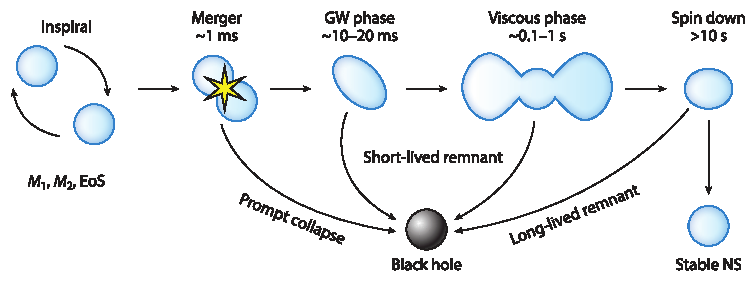
\includegraphics[width=0.70\textwidth]{Fig_3_Rad.pdf}
    \caption{
        Overview of the different phases in an \ac{NS} merger and the relative timescales. 
        The inspiral ends with the merger, when the two stars start to fuse together. 
        The early \pmerg{} evolution is entirely driven by hydrodynamics and by \ac{GW} emission. 
        If the remnant does not collapse within ${\sim}10-20\,$ms, \ac{GW} losses
        subside and other physical processes become more important: 
        Angular momentum redistribution (which is due to turbulent viscosity) 
        and neutrino losses operate over a timescale of a tenth of a second to a few
        seconds. This is also the characteristic timescale for the evolution of the remnant disk. 
        If the remnant does not collapse over a timescale of a few seconds, then it will 
        spin down because of \ac{MHD} effects over a possibly much longer timescale 
        of several seconds to a few hours. 
        (Adapted from \citet{Radice:2020ddv}).
        \red{REDO THIS FIGURE}
    }
    \label{fig:intro:RadFig1}
\end{figure}

%\footnote{
%    The orbital speed can be written as $\upsilon_{orb}\eqsim\Omega r\eqsim\sqrt{GM/(R_A + R_B)}$
%    that for equal mass binary is $\upsilon_{orb}/c\eqsim\sqrt{C}\eqsim0.39(C/0.15)^{1/2}$.
%    The radial velocity is beven by the evolution of the orbital frequency, as 
%    $\omega_r \eqsim 2\Omega r \dot{\Omega}/(3\Omega^2)$. The $\dot{\Omega}$ can be 
%    estimated from the fact, that orbital frequency satisfies 
%    $\dot{\Omega}_{GW}\sim(3456/125)(G\mathcal{M}/c^3)^5\Omega_{GW}^{11}$ during the 
%    inspiral. Then, the radial velocity reads 
%    \begin{equation}
%    \upsilon_r/c\eqsim\frac{192\pi}{15}\frac{G^3 M^3}{c^5(R_A + R_B)^3}\frac{q}{(1+q)^2}
%    \end{equation}
%    that for equal mass gives $\upsilon_r/c \eqsim 0.0034 (C/0.15)^3$.
%}.
%Merger time, $t_{merg}$, estimated from the \ac{GW} frequency at \acp{NS} collisition 
%for comparable \ac{NS} masses is given by 
%\begin{equation}
%    t_{merg}\eqsim\frac{1}{2f_{GW}^{contact}}\eqsim1.50\text{ms}\Big(\frac{M}{2.8\,\Msun}\Big)^{1}
%\end{equation}
%where the frequency of \acp{GW} when \acp{NS} come into contact, \ie, when the distance 
%between them, $r = R_A + R_B$ can be evaluated from the Kepler law, given by 
%the quadrupolar gravitoelectric term, % Eq.~7
%$2GM\Omega \eqsim 2(M_B/(MC_B) + M_B/(MC_B))^{-3/2}$ \cite{29},
%as 
%\begin{equation}
%    f_{GW}^{contact} \eqsim 1.327 \Big(\frac{C}{0.15}\Big)^{3/2}\Big( \frac{M}{2.8\,\Msun} \Big) \text{ kHz}
%\end{equation}

At the end of the inspiral \acp{NS} merge. 
%the dynamics of the system becomes significantly 
%more complex, as temperature and density rise by orders of magnitude and new 
%physical effects, \eg, magnetic fields and weak interaction, start to influence the evolution. 
%The \pmerg{} phase is not well understood and mainly explored with miltiphsyics \ac{NR} 
%simulations with various degrees of sophistication and resolution.
The system's subsequent evolution can take one of the possible trajectories 
depicted in Fig.~\ref{fig:intro:RadFig1}. Overall, the early \pmerg{} phase is 
charaterized by strong \ac{GW} emission and hydrodynamic effects. 
On a longer timescale, \ac{MHD} stresses contribute to the angular momentum redistribution, 
while neutrino emission alters the matter composition and cools it.
%
If a \ac{BH} does not form, the \ac{MHD} torques and residual \ac{GW} 
emission spin down the \ac{NS} remnant. 


%\subsection{Dynamics and Thermodynamics Conditions} \label{sec:intro:remnant}
The dynamics of the system at merger is governed by the star's orbital motion. As such, 
more compact stars (with lower $\tilde{\Lambda}$), experience more violent mergers. 
%
At collision, the \acp{NS} cores plunging into the lower density matter of the companion, 
squeezing past each other, inducing the first wave of gravity-driven compression. 
The maximum values of temperatures and densities are reached than \citep{Perego:2019adq}. 
As nuclear and centrifugal forces start to dominate, the cores bounce back until gravity 
takes over once again. This is referred to as core \bnc{} \citep[\eg][]{Radice:2018pdn}. 
%
%Notably, formed in the violent, fast collision, the remnant core, while being far from 
%hydrodynamic equilibrium, does not exhibit shocks. This is due to high speed of sound 
%of nuclear matter at supra-nuclear densities.

Formed at the remnant \ac{NS} surface, shocks are able to accelerate a fraction of matter 
to mildly-relativistic velocities. 
Inside the remnant \ac{NS}, however, shocks do not form due to high speed of sound, 
and withing the remnant, matter remains cold throughout the merger with 
the excpetion of the interface between 
two merged cores, where compression and shear dissipation raises the temperature 
to $T\sim70-110\,$MeV.
%This is accompanied by the formation of the generic structure, described
%by a pair of rotating hot regions, offset by $\sim\pi/2$ with 
%respect to dense cold regions \citep{Kastaun:2016yaf}.
%
Thus, the newly born \ac{NS} remnant is not hydrodynamically stable. 
Its dynamics is characterized by the pronounced $m=2$ bar- and $m=1$ one-armed-
deformations \citep[\eg][]{Radice:2016gym}.
%
Notably, the former leads to the strong \ac{GW} emission 
in ${\sim}10-20$~ms \pmerg{}. The backreaction from the energy and angular momentum 
loss dumps the $m=2$ mode efficiently and \ac{GW} emission subsides. 
%
This phase of evolution is sometimes referred to as \ac{GW}-dominated \pmerg{} phase.


After the emission of \acp{GW} subsides, the \ac{NS} remnant may still have an excess 
in angular momentum and gravitational mass with respect to the cold, 
rigidly rotating equilibrium with the same baryoinc mass \citep{Radice:2018xqa}. 
In other words, the object can be supported against collapse by differential rotation.
%
Its subsequent remnant evolution proceeds towards more axisymmetric configuration 
close to the limit that a rigidly rotating \ac{NS} can have.  
However, it can be interrupted at any moment by a \ac{BH} formation. %, the mass-shedding limit. 
Depending on the lifetime of the \ac{NS} remnant we distinguish \textit{long-lived}
and \textit{short-lived} ones. 
However, would a \ac{NS} remnant reach a stable state 
or collapse to a \ac{BH} depends on the 
details of \pmerg{} conditions and on the temperature and composition effects.


%%%% Disk Foramtion
The matter outside the bouncing cores, lifted by tidal torques and squeezed out at the 
collisional interface, forms a disk (or a torus). 
%
This is gravitationally bound matter, that is distinguished from the remnant by 
a sharp change in hydrodynamic quantities.
%
%Due to various contributions with different properties, the disk is highly non-uniform.
%The overall properties of the disk, such as mass, have complex dependency on 
%binary parameters, that can be expressed, at a first approximation, via fitting 
%formulae to \ac{NR} simulations \citep{Radice:2017lry,Radice:2018xqa,Radice:2018ozg}. 
The evolution of the disk as it interacts with the \ac{NS} remnant consists of 
quasi-adiabatic expansion of its outer layers 
%with $T^3/\rho^3\sim\text{const}$ as the \ac{EOS} is dominated by non-relativisitc baryons
and cooling of the inner regions. 
%
Additionally, the dynamical instabilities in the remnant inject energy and 
angular momentum into the disk. This process manifests itself in a form of spiral waves, 
propagating through the disk. 


%%%% Disk Settling down 
Withing the conditions of the \pmerg{}, weak processes take place. 
Together with spiral density waves they cool and shock periodically the 
fluid, bringing the disk to the configuration with an overall smooth 
temperature profile 
%from $\sim10\,$MeV at $\rho\eqsim10^{13}$\gcm to $\sim0.1\,$MeV at $\rho\eqsim10^4$\gcm
%with entropy $\in(3,10)$ $k_B$/baryon
and quasi-Keplerian orbit.
%
%%%% IF BH forms
Notably, if a \ac{BH} does form, the densest part of the disk is 
accreted on the dynamical timescale, which shrinks the disk and reduces its total mass by half 
%and the disk maxiumum density to $\sim10^{12}\,$\gcm,
\citep{Perego:2019adq}.


%%%% Magnetic fields
%While \acp{MF} are not expected to affect the \ac{BNS} inspiral, their influence 
%on the \pmerg{} evolution can be strong \citep{Duez:2006qe,Kiuchi:2017zzg}, as they get amplified 
%to the values exceeding that of a magnetar 
%%$10^{16}\,$Gauss, 
%by a variety of processes, 
%\eg, flux freezing and compression, \ac{KHI} at the collisional interface \citep{Kiuchi:2015sga},
%\ac{MRI}, \citep{Duez:2006qe,Kiuchi:2017zzg} and \ac{MF} winding \citep{Duez:2006qe},
Whether the ordered, large-scale \acp{MF} can form in \pmerg{} environment 
via the dynamo process is presently unknown. They are important in producing 
polar collimated outflows, jets \citep{Bucciantini:2011kx,Ruiz:2016rai} and mildly relativistic 
outflows \citep{Metzger:2018qfl,Fernandez:2018kax}. Random magnetic fields are also 
relevant for the \pmerg{} evolution, as they generate stresses, enhancing angular momentum transport. 
Presently, these processes are not well understood, as seed \ac{MHD} instabilities operate 
on small scales (centimeters) and cannot be resolved in global \ac{MHD} \ac{BNS} merger 
simulations.
%with reslistic initial condiitons
%To be able to resolve the instabilities (to increase their scale), the seed \acp{MF} are 
%artificially enhanced to the magnetar-strength \citep{Kiuchi:2015sga,Kiuchi:2017zzg}.


%%%%% Alpha-viscosity model
%The effect of \acp{MF} on the angular momentum transport can be approximated via 
%the $\alpha$-viscosity model \citep{Shakura:1972te}, calibrated 
%with very high resolution \ac{MHD} simulations \citep{Radice:2017zta,Radice:2020ids}. 
%%\red{More on it? For the theiry and GRLESS model?}
%These effects are important 
%in determining the remnant structure, lifetime and hence, the \pmerg{} \acp{GW} 
%\citep{Radice:2017zta,Shibata:2017xht} 
%%The timescale for the angular momentum redistribution in the remnant \cite{80} 
%%\begin{equation}
%%    t_{rem} \eqsim \alpha^{-1}R_{rem}^2\Omega_{rem}c_s^{-2}\eqsim 0.56\,s\Big(\frac{\alpha}{0.001}\Big)^{-1}\Big(\frac{R_{rem}}{15\,\text{km}}\Big)^2 \Big( \frac{\Omega_{rem}}{10^4\,\text{kHz}} \Big) \Big(\frac{c_s}{0.2\,c}\Big)^{-2}
%%\end{equation}
%%where $\Omega_{rem}$ and $c_s$ are the angular momentum and sound speed respectively.
%as the loss of angular momentum brings the remnant closer to either stable, 
%rigidly rotating configuration or collapse \citep{Hotokezaka:2013iia}. 
%%
%The \acp{MF} effects within the Keplerian disk facilitate accretion 
%\citep{Fernandez:2015use,Fujibayashi:2017puw,Fernandez:2018kax,Miller:2019dpt}.
%%on a timescale
%%\begin{equation}
%%    t_{disk} = \alpha^{-1}\Big(\frac{H}{R}\Big)^{-2}\Omega^{-1}_K \eqsim 0.78 \Big(\frac{\alpha}{0.02}\Big)^{-1}\Big(\frac{H/R}{1/3}\Big)^{-2}\Big(\frac{M_{rem}}{2.5\,\Msun}\Big)^{-1/2}\Big(\frac{R_{disk}}{100\,\text{km}}\Big)^{3/2}
%%\end{equation}
%%where $M_{rem}$ is the mass of the central remnant and $R_{disk}$ is the radial 
%%scale of the disk.


%%%% Neutrinos
The prime cooling mechanism in the post-\ac{GW}-dominated phase is the emission of 
neutrinos produced in hot, dense areas of the disk and remnant, and that are 
able to escape \citep{Eichler:1989ve,Rosswog:2003rv,Sekiguchi:2011zd}. 
%The typical neutrino mean free path is 
%\begin{equation}
%    \lambda_{\nu} = \Big(n_B\sigma_0(E_{\nu}/m_e c^2)^2\Big)^{-1}\simeq 24.6\,\text{m}\,(\rho/10^{14}\,\text{g}\,\text{cm}^{-3})^{-1}(E_{\nu}/10\,\text{MeV})^{-2},
%\end{equation}
%where $n_B$ is the density of baryons, and 
%\begin{equation}
%    \sigma_0 \simeq 4G_{F}^2 (m_e c^2)^2 / (\pi(\hbar c)^4)\simeq 1.76\times 10^{-44} \, \text{cm}^2
%\end{equation}
%is the typical neutrino cross section scale, and $E_{\nu}$ is the neutrino energy.
%Considering the charactersitic remnant temperature as  $T_{rem}\simeq20\,$MeV 
%energy of the thermal neutrinos then $E_{\nu}\simeq 3.15T_{rem}$ and optical depth 
%$\tau_{\nu}\simeq R_{rem}/\lambda_{\nu}=\mathcal{O}(10^{4})$.
The neutrinos are radiated on a diffusion timescale \citep{Perego:2014fma}.
%\begin{equation}
%    t_{diff} \simeq \frac{\tau_{\nu}R_{rem}}{c}\simeq 4.28\,s\Big( \frac{R_{rem}}{15\,\text{km}} \Big)^{-1}\Big(\frac{M_{rem}}{2.5\,\Msun}\Big)\Big(\frac{T_{rem}}{20\,\text{MeV}}\Big)^2.
%\end{equation}
%
%
%%%% neutrinos in the remnant and disk
Within the remnant \ac{NS}, neutrinos are in a weak and thermal equilibrium with matter. 
%due to charged current reactions. 
There, the production of electron neutrinos, $\nu_e$,
is suppressed by degeneracy, and as chemical potential $\mu_n-\mu_p+\mu_e<0$ at high temperatures, 
the electron anti-neutrinos, $\bar{\nu}_{e}$, dominate. 
Within the optically thick environment of the remnant, the effect of these neutrinos 
on the remnant evolution was found to be comparatively weak 
\citep{Foucart:2015gaa,Perego:2019adq}.
%
Within the disk, however, the optical depth for neutrinos is ${\simeq}1$ so 
they can diffuse out on a timescale of milliseconds, lowering the disk 
temperature 
%The cooling rate is controlled by the degeneracy state of neutrinos 
%that is kept at mild values by the feedback negative effect, higher 
%values have on the cooling rate.
%\citep{Beloborodov:2008nx}.
\citep{Beloborodov:2008nx}.


During the early \pmerg{}, the luminosity of the electron antineutrinos 
exceeds that of the electron neutrinos, 
%$L_{\bar{\nu}_e} \gtrsim L_{\nu_e}$, 
as the 
free neutrons are abundant in the disk and the absorption opacity for $\nu_e$ 
exceeds that of $\bar{\nu}_e$. 
%
The maximum values of fluid temperature in the disk are reached within 
the spiral waves. During the \pmerg{} evolution, the disk expands and 
cools via neutrino emission.
High temperatures lead to the electron-positron pair creation, 
%% [added from Shibata Review paper]
facilitating the positron capture by free neutrons 
%$n+e^+ \rightarrow p +\bar{\nu}_e$ 
in the disk.
%
The average particle energies are large, close to the mass difference between 
neutron and proton. The entropy per baryon varies between $3$ and 
$\lesssim  10\,$$k_{B}$/baryon \citep{Perego:2019adq}. 
In combination with the high $\nu_e$ and $\bar{\nu}_e$ luminosities, the large number 
of available positrons leads to an increase in the fluid electron fraction, 
$Y_e$, in relation to the initially neutron-rich material \citep{Qian:1996xt}.
This process is called deleptonization. %\citep[\eg][]{Perego:2014fma,Endrizzi:2019trv}
%
Additionally, a \ac{NS} remnant itself is a strong neutrino emitter. 
The neutrino irradiation of the surrounding area alters its composition, 
as neutrons and protons absorb the neutrinos,
$n+\nu_e\rightarrow p + e^{-}$ and $p + \bar{\nu}_e\rightarrow n + e^+$.
This drives the neutron and proton fraction towards equilibrium, and raises the $Y_e$.
%\red{paper says: 
%    The electron fraction is reset by an initial excess of electron antineutrino emission
%    and electron neutrino absorption,}
%% ---
If a \ac{NS} remnant collapses to a \ac{BH}, the main source of neutrinos shuts down.  
%the inner part of the disk accrets rapidly, and the disk itself settles onto 
%quasi-steady state with axisymmetric, approximately Keplerian profile. 





%Thus, alongside heating and decompression, the initially cold matter in weak 
%equilibrium, undergoes \textit{leptonization} 
%The heavy neutrinos, $\nu_{\mu,\tau}$, are balanced by pair processes and 
%decouple from matter at higher densities and temperatures within the remnant
%namely $\rho\gtrsim10^{13}$\gcm and $T\gtrsim8\,$MeV 
%\citep{Perego:2014fma,Endrizzi:2019trv},
%The, BNS simulations including
%neutrino transport predict the mean neutrino energies at infinity
%$E_{\nu_{e}}(\sim 10\,\text{MeV})\lesssim E_{\bar{\nu}_e}(\sim 15\,\text{MeV}) \lesssim E_{\nu_{\mu,\tau}}(\sim 20\,\text{MeV})$. Notably, binaries with higher mass 
%show higher neutrino energies \cite{14,86}.
%\ie, $n+\nu_e\rightarrow p + e^-$, 
%where $n$ is a neutron, $p$ is a proton and $e^{-}$ is an electron. 
%\red{check that, from Wiki}


%Neutrinos with different energies decouple from matter in different regions.
%%due to the stron dependency of the cross section on the incoming neutrino energy.
%Mildly energetic $\nu_{e}$ and $\bar{\nu}_e$ decouple at ${\sim}10^{11}\,$\gcm, found 
%in the disk, while low energy neutrinos decouple at higher ${\sim}10^{13}\,$\gcm.
%The geometric surface along which neutrinos decouple is usually called ``neutrino 
%surface'' \citep{Perego:2014fma,Endrizzi:2019trv}.
%%The dependency of the location and the geometry of this surface on the thermodynamics 
%%conditions and neutrino energy facilitates the need to coherent treatment of the 
%%strong and weak interactions over a broad span of densities and temepratures.
%%The energy dependent (spectral) neutrino radiation trasport is required in 
%%\ac{BNS} merger simulations


%%%%% Neutrino oscillations
%While it has been shown that neutrino flavor conversions may occur in the \ac{BNS} 
%\pmerg{} environment, \eg, the matter-neutrino oscillations, induced by the 
%the fact that $\bar{\nu}_e$ decouple at smaller radii then $\nu_{e}$ 
%\citep[\eg][]{Zhu:2016mwa,Tian:2017xbr}, and fast-flavor conversions above the 
%neutrino surface \citep{Wu:2017drk}, their impact on the properties of the ejected 
%material remains largely unexplored.
%%More works of neutrino quantum kinetics equations \cite{90,91}, that include 
%%collisional integral and angular and energy distributions of neutrinos are required.


%%%% EOS 
The \pmerg{} dynamics and, ultimately, the remnant's fate, depend sensibly on the 
\ac{NS} \ac{EOS}, and especially on its 
high density part. 
%
The \ac{NS} \ac{EOS} is currently not well constrained. For instance it is unknown, 
whether during the merger new particle species can form, changing the \ac{EOS}
\citep[\eg][]{Fore:2019wib,Vidana:2010ip}. 
%One of the main unknowns with respect to \ac{BNS} mergers, is the high density part, 
%%$\rho \gtrsim \rho_0$ 
%of the \ac{NS} \ac{EOS} \citep[\eg][]{Hebeler:2013nza,Oertel:2016bki}, that corresponds to the 
%relevant thermodynamic degrees of freedom and nucleonic interactions. 
%For instance, 
%the emergence of the new species, \eg, hyperons, pions, muons, and nuclear 
%resonances, would lower the matter degeneracy, and thus, soften the \ac{EOS} \citep[\eg][]{Fore:2019wib,Vidana:2010ip}.
%Additionally, the emergence of the deconfined quark matter, due to \ac{QCD} phase transition,
%would alter \ac{EOS} at very high temperatures and densities,
%the effect that is not well understood \citep{Busza:2018rrf}.
The \ac{EOS} effects on the system dynamics can be quantified with $\tilde{\Lambda}$, 
and it is common to discuss the \ac{EOS} in this context as being 
\textit{softer} or \textit{stiffer} if the $\tilde{\Lambda}$ is larger or smaller. 
%
%\subsubsection{Fate of the Remnant}
%
Another quantity describing the \ac{EOS} is the maximum supported mass of a 
non-rotating \ac{NS}, $M_{\rm max}^{\rm TOV}$ \citep{Shibata:2016}.
%
Thus, the remnant fate depends on the binary parameters, $\tilde{\Lambda}$, 
$M_{\rm max}^{\rm TOV}$, 
and finite temperature and non-beta-equilibrium composition effects 
(beta-equilibrium is the condition at which $\mu_n = \mu_p+\mu_e$).


The \ac{BH} formation directly at merger is usually referred to as \ac{PC}. 
The conditions for it are not well understood. 
Simulations show that in equal mass binaries, \ac{PC} occurs if the total mass 
exceeds a certain fraction, $1.3-1.7$, of the $M_{\rm max}^{\rm TOV}$ 
\citep{Shibata:2005ss,Shibata:2006nm,Hotokezaka:2011dh,Bauswein:2013jpa}.
%Meanwhile, simulations of unequal mass binaries show that the threshold is 
%lower \citep{Bauswein:2017vtn}, and $k_{thr}\propto C_{1.6}$, with $C_{1.6}$ 
%being the compactness of the $1.6\,\Msun$ 
%\ac{NS} \citep{Hotokezaka:2011dh,Bauswein:2013jpa,Bauswein:2017vtn}. 
%
%As \ac{PC} cases are 
%not expected to ejecta large amount of material and be \ac{EM}-loud (in case of 
%comparable mass binary), the \GW{} is believed to be not a \ac{PC} case, 
%\cite{Margalit:2017dij,Bauswein:2017vtn}. 
%
Notably, \ac{BNS} mergers that experience \ac{PC} are not expected to eject large 
amount of material and are generally though of as being \ac{EM}-quiet 
\citep{Margalit:2017dij,Bauswein:2017vtn}. 


A remnant that does not undergo \ac{PC} is a massive \ac{NS}, temporarily supported 
against collapse by the fast rotation  \citep{Baumgarte:1999cq,Rosswog:2001fh,Shibata:2006nm,Bernuzzi:2015opx}.
Its lifetime depends intricately on the \ac{EOS}, finite temperature effects, viscosity,
and is currently very uncertain.
A commonly adopted classification, based on the properties of equilibrium models (neglecting the 
dynamical, finite temperature, and magnetic effects), \ie, considering only 
$M_{\rm max}^{\rm TOV}$ and $M_{\rm max}^{\rm RNS}$\footnote{
    $M_{\rm max}^{\rm RNS}$ is the maximum mass of a rigidly rotating \ac{NS} (no differential 
    rotation) supported by zero-temperature (cold) \ac{EOS}. 
    Also sometimes referred as mass-shedding limit.
    % $M_{max}^{TOV}$ and $M_{max}^{RNS}$ are agnostic to thermal or magnetic eects 
    %which can impact the stability of the remnant in nontrivial ways (108, 72)
}, 
distinguishes between 
(i) \ac{HMNS} if $M>M_{\rm max}^{\rm RNS}$, 
(ii) \ac{SMNS} if $M_{\rm max}^{\rm TOV} \leq M_{\rm max}^{\rm RNS}$,
and (iii) stable \ac{MNS} if $M < M_{\rm max}^{\rm TOV}$ \citep[\eg][]{Baumgarte:1999cq}.
A \ac{HMNS} is supported by differential rotation that viscosity reduces with time,  
and it is expected to collapse to a \ac{BH}. A \ac{SMNS} can avoid the collapse 
even after reaching rigidly rotating configuration. The lifetime of a \ac{HMNS} and 
a \ac{SMNS} depends on the efficiency of mass and angular momentum loss 
due to, \eg, \acp{GW} and massive winds 
%and finite temperature effects 
\citep{Radice:2018xqa}. 
%
%Discussing the \ac{NR} simulations we shall distinguish between \textit{short-lived} remnants, 
%that collapse to \ac{BH} during \ac{GW}-dominated phase, 
%% taht correspods to ${\sim}10-20\,$ms after merger \cite{107,60}
%and \textit{long-lived} remnants otherwise.

%If a remnant can achieve rigid rotation, its evolution then is characterized by the emission 
%of \acp{GW} (due to residual asphericity) and magnetic braking, reducing further its 
%angular momentum, until either a \ac{BH} forms, or a stable non-rotating equilibrium is reached.
%The observations of \acp{SGRB} with X-ray plateu 
%\citep{Zhang:2000wx,Lasky:2015lej,Fan:2013cra}, which if indeed is a consequence of 
%a magnetar activity\footnote{
%    There are other possible explanations behind the X-ray plateu emission of \acp{SGRB} 
%    \citep{Oganesyan:2019jij}
%}, suggest that the remnant may survive from seconds to hours \citep{Fan:2013cra,Ravi:2014gxa}.
%Most of the energy, ${\sim}10^{52}\,$erg, that a remnant needs to lose before collapsing, if indeed \ac{SGRB} is powered by the accretion onto a \ac{BH}, 
%is believed to be carried away in form of \acp{GW}, as \ac{EM} observations of \GW{} suggest.
%%This emission can be observed for the nearby event \cite{111}, priding direct information 
%%on the remnant fate. However this emission was not observed for \GW{} \cite{67,68}

From \ac{EM} observations of the merger the fate of the remnant can be inferred, 
albeit in the model-dependent way. In case of \GW{}, the presence of \ac{EM} counterparts 
strongly disfavors \ac{PC}, as in that case the ejection of any significant amount 
of matter is not expected \citep{Margalit:2017dij,Bauswein:2017vtn,Radice:2017lry}, 
while leaving the question whether it was \ac{HMNS} or \ac{SMNS} open
\citep{Margalit:2017dij,Ai:2018jtv}. 
%
%\citet{Margalit:2017dij} suggested that the remnant was short-lived, on account of 
%the non-detection of the expected ${\sim}10^{52}\,$erg, 
%from the spin-down of the long-lived one. Assuming thus that \GW{} produced a \ac{HMNS}, 
%allows to put a constraint $M_{max}^{TOV} \lesssim 2.2\,\Msun$ \citep{Margalit:2017dij}.
%
%On the other hand, if the magnetar model of \acp{SGRB} is applied to \GW{} 
%\citep{Ai:2018jtv,Li:2018hzy,Piro:2018bpl}, the remnant is required to be long-lived
%(${\sim}$months) and exhibit weak dipol \acp{MF} \citep{Ai:2018jtv}, leading to a different 
%constraint on the maximum mass of the non-rotating star, $M_{max}^{TOV} \gtrsim 2.2\,\Msun$. 
%
%%and up to an order of magnitude lower ejecta mass ${\sim}10^{-3}\,\Msun$, that is attributed 
%%to reducied amount of emergy from radioactive decay is required to explain the observed 
%%UV/optical/infrared observations \cite{16}. 
%%There have been indications of the X-ray flaring activity in \GRB{} \cite{117}, but 
%%follow-up observations did not confirm it \cite{118}


%\subsection{Ejecta, \nuc{}, electromagnetic counterparts}

%% -------------------------------
\subsection{Ejecta}\label{sec:intro:ejecta}

%%%% Ejecta
%Generally, the ejecta is classified based on the timescale over which it occurs. 
%The \textit{dynamical ejecta} is generally divided into 
%the cold, low-$Y_e$, \textit{tidal}, produced by strong tidal torques at merger 
%and prominent in very assymetric binaries
%\citep{Rosswog:1998hy,Radice:2016dwd,Dietrich:2016hky},
%and shock-heated, high-$Y_e$, \textit{shocked}, produced 
%by the core \bnc{} induced shock waves, propagating through the \pmerg{} debris 
%\citep{Radice:2018pdn}. %Hotokezaka:2013b, Bauswein:2013yna, Sekiguchi:2016bjd, Dietrich:2016hky,
%
%The ejecta mass and velocity, as estimated by \ac{NR} simulations, lie in 
%$(10^{-4}-10^{-2})\,\Msun$ and $(0.1-0.3)\,c$ respectively 
%\citep{Hotokezaka:2013b,Bauswein:2013yna,Sekiguchi:2016bjd,Radice:2018pdn}.
% Depending on the binary \mr{} (that determins the relative controbutions of two
%components of the dynamical ejecta The outcome of the \rproc{} in the dynamical ejecta is 
%broadly consistent with the solar \rproc{} abundances.

%%%% Secular ejecta
%On a longer, \textit{secular}, timescale additional matter is ejected in a form of 
%massive winds \citep{Lee:2009,Perego:2014fma,Fernandez:2015use,Siegel:2017nub,
%    Fujibayashi:2017puw,Fernandez:2018kax,Miller:2019dpt}, % & Nedora V, et al. Astrophys. J. 886:L30 (2019)
%that could could be more massive than dynamical one, liberating $(10-40)\%$ of the disk mass. 
%%according to the numerical simulations of the disk evolution 
%%(see \eg, \citet{Radice:2018xqa} for estimates). 
%Various mechanisms contribute to 
%the matter ejection, \eg, neutrino irradiation of the polar region, generating high-$Y_e$, 
%low-mass winds \citep{Perego:2014fma,Miller:2019dpt}; nuclear recombination in the outer 
%part of the disk (after it expanded due to viscous and thermal processes) that can eject 
%${\sim}(10-20)\%$ of the disk mass at ${\sim}0.1\,c$ \citep{Lee:2009,Fernandez:2015use,Fahlman:2018llv};
%and \ac{MHD} effects facilitating matter ejection \citep{Fujibayashi:2017puw,Radice:2018xqa}.
%% & 141 Nedora V, et al. Astrophys. J. 886:L30 (2019)

%%%% Ejecta -> EM signal
%The \pmerg{} disk and remnant properties, and the lifetime of the latter, set by the 
%binary parameters and \ac{EOS} (see Sec.~\ref{sec:intro:remnant}) \citep{Radice:2018xqa,Perego:2019adq} 
%determine the properties of the secular ejecta and hence, the \ac{kN} signal 
%\citep[\eg][]{Radice:2018pdn}.
%%The disk mass dependency on the \ac{EOS} and the remnant lifetime was examined in \cite{72,70},
%%where it was pointed out that short-lived remnant is usually associated with less massive disk.
%Additionally, the presence of the remnant modifies the ejected material by means of 
%neutrino irradiation \citep{Fernandez:2015use}, providing a possibility to infer the nature of 
%the remnant from \ac{EM} observations. Modeling this process, however, requires very long-term 
%$3$D ab-initio \ac{BNS} merger simulations with complete physics, that are absent in presence.

%%%% GW170817 EM signature
%\ac{EM} followup of \GW{} showed the presence of both blue and red \acp{kN}\footnote{
%    See, however, \citet{Waxman:2017sqv} for a different interpretation
%} \citep{Villar:2017wcc}.
%Simplified \ac{kN} fitting models suggest that former requires ${\sim}0.02\,\Msun$ of high-$Y_e$ 
%material ejected at ${\sim}0.25\,c$, and the latter requires ${\sim}0.04\,\Msun$ of low-$Y_e$ 
%material ejected at ${\sim}0.1\,c$. Due to its large mass, the red component is 
%generally thought to originate in secular ejecta with the contribution from the dynamical, while 
%the origin of the blue component is less clear. Specifically, the required amount of high-$Y_e$,
%material (that is somewhat lower if sophisticated radiation transport \ac{kN} models are considered),
%is in tension with the \ac{NR} \ac{BNS} merger simulations 
%\citep{Sekiguchi:2016bjd,Siegel:2019mlp,Perego:2017wtu,Kawaguchi:2018ptg}.
%Additional ejection mechanisms have been proposed to address the discrepancy, \eg, 
%magnetic effects prior to merger \citep{Metzger:2018qfl,Fernandez:2018kax,Radice:2018ghv}. 
%%\gray{spiral waves shocking the accretion 
%%    disk by a long-lived \ac{NS} remnant \cite{141 Nedora V, et al. Astrophys. J. 886:L30 (2019)}}. 
%Future observations and long-term multiphysics \ac{NR} models will undoubtedly shed more light on this tension \citep{Metzger:2018qfl}.

%%%% Fast tail of the ejecta -- UV precourser
%\ac{NR} simulations show that within the velocity distribution of the dynamical ejecta, 
%there is ${\sim}(10^{-6}-10^{-5})\,\Msun$ of matter ejected at ${\sim}0.8\,c$ 
%\citep{Metzger:2014yda,Hotokezaka:2018gmo,Radice:2018pdn,Radice:2018ghv}, due to shocks launched 
%at core bounces \citep{Radice:2018pdn}.
%This matter is sufficiently fast to avoid the neutron capture on seed nuclei 
%%(see Sec.~\ref{sec:intro:nucleo}) 
%and will eventually undergo free-neutron decay, emitting 
%\ac{UV} radiation on a timescale of hours \citep{Metzger:2014yda}. 

%%%% Synchrotron remnant
%Expanding into the \ac{ISM}, \ac{BNS} merger ejecta generates shocks that amplify 
%random magnetic fields and accelerates electrons that in turn emit non-thermal radiation 
%via synchrotron mechanism (see Sec.~\ref{sec:intro:afterglows}). This \ac{kN} afterglow 
%can be observed on a very long, 
%moths to years, timescale \citep{Nakar:2011cw,Hotokezaka:2018gmo} and provide information 
%about merger dynamics and ejecta properties quasi-independent of uncertainty in \rproc{} \nuc{} 
%affecting the thermal, \ac{kN}, emission. 
%%
%Since ${\sim}160\,$days after the merger the non-thermal emission from \GW{} have been 
%consistent with \ac{SGRB} afterglow. However, ${\simeq}1243\,$days after the merger, a 
%change in spectral and temporal behaviour of the afterglow was observed, one of the 
%possible explanations of which is the emergence of the \ac{kN} afterglow\footnote{
%    See however \citet{Troja:2021xsw} for the alternative explanation
%} \citep{Hajela:2021faz}.
%The exact nature of this change remains at present unclear. 




%%%% DYNAMICAL EJECTA
Tidal interactions and shocks exerted upon the \acp{NS} at merger trigger the 
ejection of material on the dynamical timescale. This is the \ac{DE} \citep[\eg][]{Hotokezaka:2013b,Bauswein:2013yna,Radice:2016dwd,Radice:2018pdn},
composed of a tidal an shocked components as follows. 
%
Shortly before and during the merger, the outer parts 
of the \acp{NS}, opposite to the collisional interface, are stripped 
away by the tidal torque and centrifugal forces, forming the tidal 
component of the \ac{DE}. It is more massive in binaries with 
larger \mr{} and is maximum in those that experience tidal disruption 
\citep[\eg][]{Radice:2018pdn,Bernuzzi:2020txg}.
%%
%Such ejecta is neutron rich, confined largely to the orbital plane and exhibits 
%a crescent-like azimuthal structure \citep{Bernuzzi:2020txg}.
%
Overall, the tidal ejecta component is mostly equatorial and its 
velocity is related to the \acp{NS}' velocity at merger. 
%and the system's escape velocity, and is $\sim0.2$~c.
%
\ac{NR} simulations suggest that the ejecta mass and velocity 
lie in $(10^{-4}-10^{-2})\,\Msun$ and $(0.1-0.3)\,c$ respectively 
\citep{Hotokezaka:2013b,Bauswein:2013yna,Sekiguchi:2016bjd,Radice:2018pdn}.
%
When \acp{NS}' cores collide and \bnc{}, shocks propagate outwards inducing 
matter ejection. Additionally, a small amount of material at the 
\acp{NS}' collisional interface is shock-heated and launched into the polar 
direction. This comprises the shocked component of the \ac{DE} 
\citep{Bauswein:2013yna,Radice:2018pdn}.
%
It is more massive and faster if \acp{NS} are more compact and they collide 
at higher velocities \citep[\eg][]{Radice:2018pdn}. 


The dynamical ejecta has a broad distribution in terms of composition, 
velocity and mass, dependent on the parameters of the binary and \ac{NS} \ac{EOS}, 
%
and thhe relation between the binary parameters and ejecta properties is still 
largely unconstrained.

\ac{NR} simulations show that within the velocity distribution of the dynamical ejecta, 
there is ${\sim}(10^{-6}-10^{-5})\,\Msun$ of matter ejected at ${\sim}0.8\,c$ 
\citep{Metzger:2014yda,Hotokezaka:2018gmo,Radice:2018pdn,Radice:2018ghv}, 
due to shocks launched at core bounces \citep{Radice:2018pdn}. 
This sometimes referred to as fast tail of \ac{DE}.
%This matter is sufficiently fast to avoid the neutron capture on seed nuclei 
%%(see Sec.~\ref{sec:intro:nucleo}) 
%and will eventually undergo free-neutron decay, emitting 
%\ac{UV} radiation on a timescale of hours \citep{Metzger:2014yda}. 


%%%% WINDS
%Various mechanisms contribute to 
%the matter ejection, \eg, neutrino irradiation of the polar region, generating high-$Y_e$, 
%low-mass winds \citep{Perego:2014fma,Miller:2019dpt}; nuclear recombination in the outer 
%part of the disk (after it expanded due to viscous and thermal processes) that can eject 
%${\sim}(10-20)\%$ of the disk mass at ${\sim}0.1\,c$ \citep{Lee:2009,Fernandez:2015use,Fahlman:2018llv};
%and \ac{MHD} effects facilitating matter ejection \citep{Fujibayashi:2017puw,Radice:2018xqa}.
As the disk expands and cools, recombination of nucleons into alpha particles 
starts to take place. The energy released in recombination might be sufficient 
for the outermost layers to become unbound, leading to a massive outflow,  
depleting the disk \citep{Beloborodov:2008nx,Lee:2009uc,Fernandez:2013tya}.
%
%\citep{Lee:2009uc,Fernandez:2015use,
%    Wu:2016pnw,Siegel:2017nub,
%      Fujibayashi:2017puw,Fernandez:2018kax,Radice:2018xqa,Fujibayashi:2020dvr}.
%
Furthermore, so-called neutrino-driven winds (\nwind{}; \citet{Dessart:2008zd,Perego:2014fma,Just:2014fka})
induced by neutrino heating above the remnant, 
are expected to contribute to the mass loss. 
%
The presence of the remnant modifies the ejected material by means of 
neutrino irradiation \citep{Fernandez:2015use}, providing a possibility to infer the nature of 
the remnant from \ac{EM} observations. Modeling this process, however, requires very long-term 
$3$D ab-initio \ac{BNS} merger simulations with complete physics, that are absent in presence.
%
Overall, analytical estimates and simulations with various approximations show that 
up tp ${\sim}40\%$ of the disk can be ejected via viscous processes with a 
typical velocity ${\lesssim}0.1\,$c \citep{Fernandez:2018kax,Radice:2018xqa}.
The ejecta is expected to be relatively slow and neutron-rich. 
%Importantly, these processes are expected to take place on timescales exceeding 
%those of our simulations. 



\subsection{$R$-process \nuc{}} \label{sec:intro:nucleo}
\red{introduce weak and full r-process}
\red{Add info on r-process trajecotry, including what are the (i) seed nuclei, }

Nuclides with atomic number  $A\geq 56$ cannot be synthesized via nuclear burning 
due to their large Coulomb barriers. They are produced via 
neutron capture processes \citep{Burbidge:1957}.
%%%% Nucleosynthesis Cites
The maximum $A$ of a nuclide is limited by its binding energy, $Q_n$. 
At $Q_n \simeq1 \,$MeV photodisintegration starts breaking nuclides apart. 
The place in the parameter space of temperature and density where this occurs 
is called \textit{neutron drip line} \citep{Rolfs:1988}.
%%%%% Fast and Slow
Nuclides produced via neutron capture are generally unstable to $\beta$-decay,
and depending on whether the timescale for the decay is slower (faster) than 
the timescale of neutron capture, one distinguish rapid (slow) process called,
\rproc{} (\sproc{}).
%
The \sproc{} moves along the valey of stability, while \rproc{} moves along the 
neutron drip line. The valley of stability being the region in nuclides chart 
where nuclides are stable to radioactive decay based on their binding energy. 
%
When a nuclide reaches a closed neutron shell configuration, the cross-section 
for the subsequent neutron capture shrinks, and capture processes suspend until 
several $\beta$-decays take place. This results in an overproduction of nuclides 
that are located at the intersection between the neutron drip line and closed 
neutron shell for the \rproc{}. This manifests as ``peaks'' in the final abundance 
pattern at $A$ corresponding to these configurations.
Closed shell nuclides are located at $N=50,\: 82, \: 126$ and 
corresponding abundance peaks $A=80,\:130,\:194$ for \rproc{}, 
with $A$ being the atomic number (see \eg, \citet{Arnould:2007gh}).

%%%% R-process mechanism
\red{introduce weak and full r-process}
\red{Add info on r-process trajecotry, including what are the (i) seed nuclei, }
\red{In which Ye what nucleo proceeds}
The outcome of the \rproc{} \nuc{} depends sensibly on the hydrodynamic properties 
of matter and its composition. 
%Such parameterized model of \citet{Lippuner:2018phd} (see their Figure 3.1) 
%allows to deduce several important trends.
%
Specifically, that at high entropy, that result in a high neutron-to-seed ratio, 
even if seed nuclei are light, full \rproc{} can occur.
At low entropy, the \rproc{} is jugged as there are not many free neutrons available,
but the presence of very heavy seed nuclei still allows for the \nuc{} to proceed. 
At high $Y_e$, where ejecta is less neutron rich, the full \rproc{} no longer occurs,  
as there are not enough neutrons per seed nucleus to reach the third peak.
However, at high entropy and low $Y_e$ the $3$rd peak element can be synthesis as, while 
there are few seed nuclei, the neutron to seed ratio is high.
%
The main quantity defining the final abundances was shown is the electron fraction.

%%%% R-proces cites
Conditions for the \rproc{} can be achieved in different astrophysical cites, \eg, 
certain types of \acp{SN} and \ac{BNS} mergers where very neutron rich (low 
electron fraction, $Y_e = 1/(1 + N_n/N_p)$, with $N_n$ and $N_p$ being the 
total proper number density of neutrons and protons respectively) 
conditions can be reached
\citep{Mathews:1990,Thielemann:2011,Lippuner:2015gwa,Siegel:2019mlp}. 

%% --- BNS :: other ejecta types
The \rproc{} is expected to take place in different types of ejecta from \ac{BNS} mergers.
In \nwind{} the neutrino irradiation can significantly increase the electron 
fraction, which, depending on the ejecta velocity, can reach the 
$Y_e\leq 0.45$ \citep{Qian:1996xt}. 
%
At this point the weak equilibrium sets in between the ejecta and neutrinos.
High electron fraction implies that only the light elements will be produced.
The numerical studies indeed support this picture 
\citep{Dessart:2008zd,Perego:2014fma,Just:2014fka,Martin:2015hxa,Foucart:2016rxm}. 

The bulk of the ejecta from \ac{BNS} mergers is expected to come in the form of 
viscous- and recombination-driven winds. This ejecta, however, is expected to take 
place over longer timescales than those of our simulations.
Studies have shown that this ejecta has a broad distribution of the electron fraction.
The \rproc{} \nuc{} within it would produce light as well as heavy elements
\citep{Fernandez:2013tya,Just:2014fka,Wu:2016pnw,Siegel:2017nub,Fujibayashi:2017puw,Fernandez:2018kax}.
The production of the heavy \rproc{} elements, however, might be supressed in these winds
if a long-lived \ac{NS} is present \citep{Metzger:2014ila,Lippuner:2017bfm}.

%% --- other types
Regarding the \acp{SN}, winds driven by strong neutrino fluxes from the hot, deleptonized
core \citep{Qian:1996xt} were suggested as a promising cite \citep{Woosley:2002,Wanajo:2006mq}.
However, high $Y_e$ found in such winds do not allow for the full \rproc{} and only ``light'' heavy 
nuclide, up to $A\sim130$, can be synthesized 
\citep{Qian:1996xt,Thompson:2001ys,Fischer:2010,Roberts:2010,MartinezPinedo:2012rb,Wanajo:2013} 
%
A full \rproc{} can be achieved in so-called magnetorotationally driven \ac{CCSN},
(a rare type of \ac{CCSN} with a rapidly spinning strongly magnetized core), 
initiated by the \ac{MRI} and accompanied by a % magnetorotational processes \eg, 
formation of a 
collimated bipolar jet 
\citep{Wheeler:2000,Akiyama:2003,Burrows:2007yx,Mosta:2014jaa,Mosta:2015,Siegel:2019mlp}.
Conditions within such a jet were found to be suffient for full \rproc{} \nuc{} 
\citep{Winteler:2012,Nishimura:2015nca}.
%The rarity of this type of \acp{SN}, 
%however, might not allow for them to be the dominant source or \rproc{} material 
%\citep{Nishimura:2015nca} 

%Neutron-rich ejecta from \ac{BNS} and \ac{NSBH} mergers are regarded as one of 
%the main cites or \rproc{} \nuc{}.
%
%Mergers of two \acp{NS} or a \ac{NS} and a \ac{BH} are regarded as one of the main cites 
%of \rproc{} material.% (See Sec.~\ref{sec:intro:bns_merg}). 

%%%% Fission cycling
Under the very neutron-rich conditions, 
the nuclides beyond $A=300$ can be produced. Being unstable to fission, they 
decay into seed nuclides shortly after formation.
However, before they reach the valley of stability, neutron capture occurs again, and the cycle repeats.
This is so-called \textit{fission cycling}.
It is maintained as long as there are free neutrons, after which nuclides decay 
for the last time, forming a remarkably robust abundance pattern independent from the 
number of cycles (and thus from the exact matter conditions) 
(see figure 4 in \citet{Korobkin:2012uy}). 

%%%% Cites
There is no consensus yet on what is the main source of \rproc{} material in the 
Universe. 
Observed \rproc{} abundances in \ac{MP} stars, formed early in the Galactic history, 
point towards a sources that was active in the early Universe, which is in tension with the long, 
$10^{6} - 10^{9}$ years, delay time required for compact object inspiral 
\citep{DeDonder:2004cx,Dominik:2012kk}. This estimate, however, depends strongly on the 
uncertain common envelop evolution phase of the massive binary (progenitors)
\citep[\eg][]{Dominik:2012kk}.
%
Observations of certain \acp{UFG} suggest that stars there have been enrighed by rare, 
high-yield events (\eg, \ac{UFG} Reticulum II showed abundances similar to solar, 
while other \ac{UFG} galaxies show $2-3$ times lower abundances) \citep{Ji:2016}.
%
Earth crust and meteorites $^{244}$Pu studies also point towards rare, high-yield 
events \citep{Wallner:2015,Tsujimoto:2017}. This estimation has been confirmed with 
models of galactic mixing \citep{Hotokezaka:2015zea}.
%
It is however difficult to explain the observed uniform distribution of \rproc{} 
elements in the Galaxy with such events \citep{Argast:2003he}.
%
Population synthesis models have indicated that with a contribution from 
magnetorotationallydriven \acp{CCSN} the compact object mergers can account for the 
observed distribution \citep{Ishimaru:2015,Cescutti:2015,Wehmeyer:2015,VanDeVoort:2015}.



%% ----------------------------------
\subsection{Kilonova}


\citet{Li:1998bw} suggested that 
radioactive decay of the material enriched with \rproc{} elements,
ejected in \ac{BNS} or \ac{NSBH} mergers, can power an \ac{EM} transient.
%
Authors showed that contrary to the normal \acp{SN}, 
the ejecta would quickly become transparent to its own emission, 
that would reach its peak on a timescale of around a few days. 
%
The main difficulty in this pioneering work was the lack of a \nuc{}
models to estimate the radioactive heating in the ejecta. 
%
Our understanding of \ac{kN} has significantly improved since then
\citep[\eg][]{Kulkarni:2005jw,Metzger:2010,Roberts:2011,Metzger:2016pju,Wollaeger:2017ahm} 
and advanced even further with the detection of \AT{} \citep[\eg][]{Metzger:2019zeh}.

The final composition of the ejecta determines its optical opacity 
which can vary by orders of magnitude if $3$rd peak elements, 
lanthanides 
%$(58\leq Z \leq71)$ 
and actinides, 
%$(90\leq Z \leq 103)$, 
are present 
due to their open $f$-shells and, thus, a plethora of 
absorption lines \citep{Tanaka:2013ana,Kasen:2013xka}.
%
The properties of the \ac{kN} emission have complex 
dependency on the properties and geometry of different components of 
\ac{BNS} merger ejecta \citep{Metzger:2019zeh}.
%
Describing the complex \ac{kN} signature it is common to 
generalize it into two main components, ``blue'' and ``red'' 
depending on whether the fraction of lanthanides and actinides is low or high.
%
The former corresponds to the high $Y_e$ material that produces emission 
that peaks in \ac{UV}/optical bands on a timescale of hours-days, 
while the latter is related to low-$Y_e$ material that generates the 
emission peaking on a significantly 
longer timescale, tens of days, in \ac{IR} and \ac{NIR} bands
\citep{Barnes:2013wka,Grossman:2013lqa,Lippuner:2015gwa}.

Both ``blue \ac{kN}'' and ``red \ac{kN}'' were observed in \AT{}, 
confirming the qualitative picture and implying a diverse composition 
of the ejected material \citep[\eg][]{Villar:2017wcc}.
%\citep{
%    Arcavi:2017xiz,Coulter:2017wya,Drout:2017ijr,Evans:2017mmy,Hallinan:2017woc,
%    Kasliwal:2017ngb,Nicholl:2017ahq,Smartt:2017fuw,Soares-santos:2017lru,Tanvir:2017pws,
%    Troja:2017nqp,Mooley:2018dlz,Ruan:2017bha,
%    Lyman:2018qjg
%}.
%
%The quantitative analysis -- the comparsion between the ejecta properties 
%inferred from the \ac{kN} models and those seen in \ac{BNS} merger simulations,
%however, showed substantial disagreement. Specifically, the \ac{BNS} merger 
%simulations under-predict the amount of ejecta. The discrepancy is attributed 
%to the insufficient length of those simulations, which does not capture long-term 
%secular ejecta. 
Semi-analytic two-components spherical \ac{kN} models to 
the \AT{} observations provided estimates for the ejecta properties 
for these two components. 
%
Specifically, for the langhinide poor (rich) \ie, blue (red) components, 
the required mass is $2.5\times10^{-2}M_{\odot}$ ($5.0\times10^{-2}M_{\odot}$) 
and velocity $0.27\,$c ($0.15\,$c) \citep{Cowperthwaite:2017dyu,Villar:2017wcc}. 
%See however \citep{Waxman:2017sqv} for an alternative interpretation.
%See also \citep{Siegel:2019mlp} for the compiled data on the \ac{kN} models.
%
%%%% Issue with blue Kilonova
The outflow properties inferred for \AT{} using multi-component semi-analytic and 
2D radiation transport \ac{kN} models including ejecta anisotropy and 
cross-component irradiation are broadly compatible with the results from 
merger simulations, \eg, \citep{Kawaguchi:2018ptg}. % see also Sec.~\ref{sec:intro:kilonova}. 
%
%\ac{EM} followup of \GW{} showed the presence of both blue and red \acp{kN}
%%\footnote{
%%    See, however, \citet{Waxman:2017sqv} for a different interpretation
%%} 
%\citep{Villar:2017wcc}.
%However, simplified \ac{kN} fitting models suggest that former requires ${\sim}0.02\,\Msun$ of high-$Y_e$ 
%material ejected at ${\sim}0.25\,c$, and the latter requires ${\sim}0.04\,\Msun$ of low-$Y_e$ 
%material ejected at ${\sim}0.1\,c$. Due to its large mass, the red component is 
%generally thought to originate in secular ejecta with the contribution from the dynamical, while 
%the origin of the blue component is less clear. 
%
However, certain disagreements remain. 
For instance, the required amount of high-$Y_e$, material 
(which is somewhat lower if sophisticated radiation transport 
\ac{kN} models are considered), is in tension with \ac{NR} \ac{BNS} merger simulations 
\citep{Sekiguchi:2016bjd,Siegel:2019mlp,Perego:2017wtu,Kawaguchi:2018ptg}.
%
Additional ejection mechanisms have been proposed to address the discrepancy, \eg, 
magnetic effects prior to merger \citep{Metzger:2018qfl,Fernandez:2018kax,Radice:2018ghv}. 
%\gray{spiral waves shocking the accretion 
%    disk by a long-lived \ac{NS} remnant \cite{141 Nedora V, et al. Astrophys. J. 886:L30 (2019)}}. 
%Future observations and long-term multiphysics \ac{NR} models 
%will undoubtedly shed more light on this tension \citep{Metzger:2018qfl}.
%% ---
Moreover, it is difficult to reproduce the early blue emission, that requires 
low opacity, massive ejecta, that is generally not found in \ac{NR} 
simulations \citep{Fahlman:2018llv}. 
%% ---
Notably, the early blue component can be explained by the emission arising 
in the interaction between a relativistic jet and the ejecta
\citep{Lazzati:2016yxl,Bromberg:2017crh,Piro:2017ayh}.
However, simulations show that that successful jets do not deposit a sufficient amount of thermal energy in the ejecta for this mechanism to work \citep{Duffell:2018iig}. 
Other possibilities include the presence of highly magnetized winds \citep{Metzger:2018uni,Fernandez:2018kax},
or the presence of the so-called viscous dynamical ejecta \citep{Radice:2018ghv}.
These two explanations require the development of large-scale strong magnetic fields.


Prior to \AT{}, there were other \ac{kN} candidates based on the 
detection of \ac{SGRB}, with infrared excess \eg, 
GRB130603B, \citep{Berger:2013wna,Tanvir:2013pia}, 
GRB060614 \citep{Jin:2015txa,Yang:2015pha}, 
GRB050709 \citep{Jin:2016pnm}.
%GRB200522A \citep{WRONG}  Bruni:2021ilp
However the exact nature of the observed signals were not well constrained. 


%% ------------------------------------------------
\subsection{Non-thermal afterglows}

\acp{GRB} are irregular pulses of gamma-ray radiation with broken power-law 
(non-thermal) spectrum, peaking at KeV-MeV \citep{Band:1993,Kouveliotou:1993,Meegan:1992xg}.
%
With respect to the duration, \acp{GRB} are split into two categories: \acp{SGRB}, 
that last ${\leq}2\,$s and long \acp{GRB} that last ${\gtrsim}2\,$s. 
%
It is generally accepted that the latter are the 
result of the collapse of massive ${\geq}15\,M_{\odot}$ stars,
 while the former, at least in part, are attributed to mergers of compact objects. 
%
However, the exact physical origin of different duration 
\acp{GRB} is not fully understood.
%
%%%% LGRB
%Indications that long \ac{GRB} are associated with core-collapse supernovae, \acp{SN}, 
%are two fold. These \acp{GRB} are typically observed in star-forming regions of their 
%host galaxies \citep[\eg][]{Bloom:2000pq,Bloom:2002hc,Fruchter:2006py,Christensen:2004yx,CastroCeron:2006jh} 
%and several \acp{GRB} are spectroscopically associated with Type Ic \acp{SN}, albeit 
%these \acp{GRB} were significantly less bright and might not be typical \acp{GRB} 
%\citep[\eg][]{Liang:2006ci,Bromberg:2011fm}. Additionally, the late time behaviour 
%of some \acp{GRB} includes a \acp{SN}-like "bump" in the optical and spectral changes 
%that might imply that underlying \acp{SN} flux becomes dominant over \acp{GRB} 
%\citep[\eg][]{Bloom:1999,Woosley:2006fn}.

%%%% Cosmology implications
\acp{GRB} are distant events, most of which were localized to outside the Local Group 
\citep[\eg][]{Mao:1992,Piran:1992,Fenimore:1993}. 
%
Particularly useful for distance estimations are the observations of \ac{GRB} afterglows 
(fading X-ray, optical and radio emission), 
that allow to estimate the Redshift \citep[\eg][]{Costa:1997cg,Frontera:1997ae}.

%%%% Mechanism of radiaiton
Analysis of the multi-wavelength afterglow data of \acp{GRB} 
\citep[\eg][]{Panaitescu:2001bx} suggested that the mechanism behind the afterglow 
emission is non-thermal. Specifically, the afterglow is attributed to the 
synchrotron emission coming from the external forward-shock, which forms 
when \ac{GRB}-ejecta sweeps-up the \ac{ISM} medium\footnote{
    The specific indications for the non-thermal origin of the emission 
    are the power law decay of the light curves, and power-law spectrum. 
%    with flux decaying as, $F_{\nu}\propto \nu^{-1}$ 
%    and power-law spectrum $F_{\nu}\propto \nu^{-0.9\pm 0.5}$.
} 
\citep{Rees:1992ek,Paczynski:1993gz,Meszaros:1993ju,Meszaros:1996sv}.
%

%%%% Jet break
%The temporal behavior of many (but not all) \acp{GRB} shows a change, a steepening 
%of the light-curve (to $F_{\nu}\propto t^{-2.2}$) at $\sim 1$~day after the burst. 
%This is usually attributed to the 
%%\gray{deceleration of the colimated GRB-outflow, jet, and decrease on the realtivisitc beaming. This in turn makes the edge of the jet visible to an observer.} 
%finite angular extend of the \ac{GRB}-ejecta, jet \citep[\eg][]{Rhoads:1999wm,Sari:1999mr}. 
%When jet decelerates and relativistic beaming decreases (and the jet edge becomes visible), 
%the optical and X-ray lightcurves decay achromatically faster. This achromatic transition 
%from slow to faster decay is called "jet-break".
%
%%% PROBLEMO -- jet-break is not a universal feature.
%Notably, this jet-break is not observed in all \acp{GRB} for the reason that is not fully 
%understood \citep[\eg][]{Fan:2006pj,Panaitescu:2006,Liang:2007ti,Sato:2006jg,Liang:2007rn,Curran:2007cp,Racusin:2008bx}
%%
%%% PROBLEMO -- GRB density seems uniform, but SSE models predict wind-like profile
%Models of the broadband emission of \acp{GRB} with jet-break showed that the 
%\ac{CBM}, is uniform with number density \red{$\sim 10^{-3}$} \citep{Panaitescu:2001bx}. 
%If \acp{GRB} produced in collapse of massive stars \citep{Woosley:1993,Paczynski:1997yg}, 
%this contradicts the expected density profile from stellar winds, \eg, $\rho\propto r^{-2}$ 
%\citep[\eg][]{Dai:1998iz,Chevalier:1999jy,Chevalier:1999mi,Ramirez-Ruiz:2001} 
%\red{this might be very outdated.}
%
%% sGRB
The origin of \acp{SGRB} was first linked to elliptical galaxies with dominant 
older stellar population 
\citep[\eg][]{Gehrels:2005qk,
%    Fox:2005kv,Barthelmy:2005bx,Berger:2005dr,Panaitescu:2005er,Bloom:2005qx,Guetta:2005bb,
    Nakar:2007yr}, 
and thus with \ac{BNS} mergers. 
%
A more direct evidence came with the detection of \ac{SGRB}, \GRB{}, 
\citep{
    %Savchenko:2017ffs,
    Alexander:2017aly,Troja:2017nqp,
    %Monitor:2017mdv,Nynka:2018vup,
    Hajela:2019mjy}, 
detected by the space observatories Fermi 
\citep{TheFermi-LAT:2015kwa} and INTEGRAL \citep{Winkler:2011}, one 
of the counterparts of \GW{} \citep{TheLIGOScientific:2017qsa}.
%
%Generally \acp{SGRB} show a complex time behavior of early afterglow X-ray emission, 
%in particular a presence of a plateau ($F_{x}\propto t^{-1/2}$), after the initial sharp 
%decrease ($F_{x}\propto t^{-3}$) which a standard forward shock model does not predict. 
%This implies that early X-ray afterglow is shaped by a variety of physical processes 
%\citep{Zhang:2005fa}.
%
%
%%%% EARLY emission problem
%Two main questions stem from these observations: is the mechanism behind the prompt 
%$\gamma$-ray emission and early afterglow emission is the same (or do they originate from 
%the same outflow), and is the early X-ray radiation produced by the external shock (just a 
%blast wave takes long time to become self-similar) or does it originate from an internal 
%shock? An indication that the long-lived central engine activity might affect the 
%afterglow came from the observed sharp increase in X-ray flux (flares) on a 
%scale of minutes to hours after the end of the \ac{GRB}
%\citep{Burrows:2005ww,Chincarini:2007fp,Chincarini:2010,Margutti:2011}, 
%which could not be attributed to the inhomogeneities in the \ac{CBM}.
%%% PROBLEMO!
%Thus, the early X-ray behaviour of \acp{GRB} $t < 10^{4}$~s post-burst is not well 
%understood and seems to be in tension with standard afterglow forward shock emission model.
%
%\textcolor{red}{
%    One of the foremost unanswered questions about GRBs is the physical mechanism
%    by which prompt $\gamma$-rays the radiation that triggers detectors on board
%    GRB satellites are produced. Is the mechanism the popular internal shock
%    model 6 \cite{(Rees and Meszaros, 1994)}, the external shock model, or something
%    entirely different? Are $\gamma$-ray photons generated via the synchrotron process
%    or inverse-Compton process, or by a different mechanism? Answers to these
%    questions will help us address some of the most important unsolved problems
%    in GRBs  how is the explosion powered in these bursts? Does the relativistic
%    jet produced in these explosions consist of ordinary baryonic matter, electron positron
%    pairs, or is the energy primarily in magnetic fields?
%}
%
%Once again, while it is suggested that the high energy emission, after the propmt phase is produced 
%by the synchrotron process in the external forward shock, \citep{Kumar:2009,Ghisellini:2010}, 
%the mechanism behind the high and low energy $\gamma$-ray emission in the prompt phase remains unknown. 
%Possible mechanisms include: inverse Compton and synchrotron emission in internal and external shocks
%\citep[\eg][]{Rees:1992ek,Dermer:1998py,Lyutikov:2003ih,Zhang:2011} and 
%photospheric radiation with contribution from multiple \ac{IC} scatterings
%\citep[\eg][]{Thompson:1994zh,Ghisellini:1998jy,Meszaros:1999gb,Peer:2005qoc,Peer:2008udu,Giannios:2006jb,Ioka:2007qk,Asano:2009gi,Lazzati:2010,Beloborodov:2010,Toma:2011}.
%
However, while the \GRB{} has confirmed that \ac{BNS} mergers are responsible 
for at least some of \acp{SGRB}, \GRB{} was dimmer than any other event of its class. 
%Different interpretations for its dimness and slow rising flux were proposed including 
%Different interpretations for this included off-axis jet, cocoon and structured jet. 
Now it is commonly attributed to the jet having lateral structure\footnote{
    Structured jet, contrary to the top-hat jet has an angular dependency of the 
    matter energy and Lorentz factor. Such structure is believed to appear 
    when jet drills its way through the merger ejecta \citep{Lamb:2017ych}.
}, which was also observed off-axis 
\citep[\eg][]{Ghirlanda:2018uyx}. 
%    Fong:2017ekk,Troja:2017nqp,Margutti:2018xqd,Lamb:2017ych,Lamb:2018ohw,
%    Ryan:2019fhz,Alexander:2018dcl,Mooley:2018dlz,
%    Ghirlanda:2018uyx
%}.
%
The \GRB{} late emission, the afterglow, provided information on the energetics of the 
event and on the properties of the \ac{ISM} \citep[\eg][]{Hajela:2019mjy}. 

%% ---------------
%% Kilonova Afterglow
%% ---------------


In addition to the \ac{GRB} beamed emission, more isotropic non-thermal,
emission is expected to arise from electrons accelerated in shocks formed between the 
mildly relativistic ejecta and the \ac{ISM} \citep{Nakar:2011cw}. 
Called, \ac{kN} afterglow, it is expected to peak in radio band and continue 
to be observable on a time scale of years 
after merger. Notably, all ejecta components contribute to the emission, 
but depending on the ejecta velocities and kinetic energy, 
the brightness in different frequencies varies. 
%
The mechanism behind this emission is phenomenologically similar to the one, 
responsible for the \ac{GRB} afterglow. Specifically, as various ejecta components 
interact with each other and with \ac{ISM}, the latter generates a long-lived blast wave. 
The formed shock, propagating upstream, amplifies random magnetic fields and accelerates 
electrons, that subsequently emit synchrotron radiation. % and \ac{SN} early remnants. 

As \ac{NR} simulations showed the presence of mildly relativistic ejecta, 
(\eg, from core \bnc{}), such emission was studied in past works 
\citep[\eg][]{Piran:2012wd,Hotokezaka:2015eja,Hotokezaka:2018gmo,Radice:2018pdn} 
and was expected in the case of \GW{} \citep[\eg][]{Kathirgamaraju:2018mac}.

Since ${\sim}160\,$days after the merger the non-thermal emission from \GW{} have been 
consistent with \ac{SGRB} afterglow \citep{Troja:2020pzf,Hajela:2019mjy}. 
However, ${\simeq}1243\,$days after the merger, a 
change in spectral and temporal behaviour of the afterglow was observed.
A change, that is not compatible with the afterglow from a structured jet. 
While exact nature of this change remains at present unclear, one 
of the possible explanations is the emergence of the 
\ac{kN} afterglow\footnote{
    See however \citet{Troja:2021xsw} for the alternative explanation
} \citep{Hajela:2021faz}.

%Notably, the observed non-thermal emission from \GW{}, was first interpreted 
%as the non-thermal emission from the ejecta \citep{Mooley:2017enz}.
%This interpretation was however disproved by the emergence of jet break
%
%
%Specifically, a strong radio emission is expected from \ac{BNS} ejecta \citep{Piran:2012wd,Hotokezaka:2015eja}. 
%The \ac{BNS} merger radio remnant is expected to peak on a time-scale 
%of ${\sim}$years after the merger.% and be visible over a similar timescale. Notably, this is 
%Assuming that the ejecta is expanding into the unshocked \ac{ISM}, as it was shown 
%that if the \ac{ISM} is pre-shocked by the jetted outflow, and the \ac{ISM} density is 
%reduced, the kilonova afterglow would be delayed. 
%
%In \citet{Piran:2012wd}, the synthetic \ac{kN} afterglow \acp{LC} are calculated 
%for a set of \ac{NR} \ac{BNS} merger simulation with properties typical to the 
%Galactic binary population and \ac{ISM} density usually found in the Galactic disk, 
%$\nism{\sim1}\ccm$. Authors showed that the from a binary of two $1.4\,\Msun$ \acp{NS}, 
%the kilonova afterglow would peak $\sim10$~years after the merger if $\nism = 0.1\,\ccm$ 
%and $\sim3$~years if $\nism = 1\,\ccm$ in radio bands, $\nu=1.4$~GGz and $\nu=150\,$MGz. 
%Notably, both values of the \ac{ISM} density are larger than what is inferred for \GW{}. 
%Indeed, jet fitting models and dependent analysis of the diffuse emission suggest 
%$\nism\in(10^{-4},10^{-2})\,$\gcm \citep{Hajela:2019mjy}.
%In \citet{Piran:2012wd} authors focus on the observational prospects of this afterglow 
%and compare it to other \ac{EM} emission expected for \ac{BNS}. 


%% =====================================================================================
%%
%%              O R G A N I S A T I O N
%%
%% =====================================================================================

\section{Aims and organization of this thesis}

As we showed above, mergers of \acp{BNS} are at the center of a variety of 
physical processes in astrophysics. And while significant work 
has been done to advance our understanding of these events, many 
fundamental questions remain. 
%
The foundation of the \ac{BNS} merger research are \ac{NR} simulations.
However, most \ac{BNS} \ac{NR} simulations available in the literature 
are ether short, typically ${\lesssim}10\,$ms \pmerg, rare, but with 
advanced physics \citep[\eg][]{Vincent:2019kor}, 
or neglect important physics, \eg, neutrino reabsorption, 
and effects of the \ac{MF}-induced turbulence \citep[\eg][]{Lehner:2016lxy}. 
% \citep[\eg][] \citep[\eg][]{Kawaguchi:2020vbf}. \cite{Lehner:2016lxy}
%
In this thesis we postprocess and analyze a large sample of new 
\ac{NR} simulations performed \wisky{} \ac{NR} code.
Our simulations include \ac{GR}, microphysical \acp{EOS} with finite-temperature 
effects, neutrino emission and reabsorption, and effects of the 
\acp{MF} on the angular momentum transport. Some of 
our simulations have been continued till ${\gtrsim}100\,$ms \pmerg{}. 
All our simulations have chirp-mass, equal to that inferred for 
\GW{}. 
%
Postprocessing and alanyzing these simulations, 
computing \rproc{} nucleosynthetic yields, 
and thermal and non-thermal \ac{EM} counterparts to mergers, 
we aim to investigate the following questions.

\begin{itemize}
    \item What is the evolutionary trajectory of a \ac{NS} remnant born with 
    an excess in mass and angular momentum with respect to the mass-shedding 
    limit, \ie, \ac{HMNS}? Does it collapse to a \ac{BH}?
    \item 
%    How the physics input of our simulations affects the ejecta properties and 
%    the resulted nucleosynthetic yields?
    Can \ac{BNS} mergers be considered as 
    the prime source of \rproc{} elements in the Universe?
    \item How the statistical properties of \ac{DE} of our simulations 
    differ with respect to other published models? What is the 
    up-to-date relation between binary parameters and ejecta properties? 
    How strongly it depends on systematics?
    \item Can the \ac{kN} produced by the ejecta from our long simulations 
    provide better explanations to \AT{}? 
    \item Is the \ac{kN} afterglow from our models consistent 
    with the changing behaviour of \GRB{} afterglow? 
\end{itemize}

Ultimately we aim to seek a possibility to further constrain the properties 
of \GW{} and \ac{NS} \ac{EOS}.


%\ac{BNS} mergers and especially the \pmerg{} evolution hosts a number of interesting 
%and yet poorly understood physics. 
%Although there are published \ac{NR} simulations of \ac{BNS} mergers, 
%most of them are either very short, or neglect important physics, \eg, 
%neutrino reabsorption, and effects of the \ac{MF}-induced turbulence. 
%Thus, \ac{EM}
%Moreover, the statistical analysis of up-to-date sample of thesis 
%simulations is a pending task.
%%
%We intend to improve upon this situation by performing a large number of long-term ab-initio 
%\ac{NR} \ac{BNS} simulations with neutrino reabsorption and viscosity, focusing on the 
%\pmerg{} evolution of the remnant and astrophysical aspects, \ie, matter ejection, 
%\rproc{} \nuc{} and \ac{EM} signals.
%%
%All simulations have chirp masses targeted to \GW{}, and with this work we aim to further 
%constrain the \ac{NS} \ac{EOS} and the properties of the binary and shed light on 
%some of the aforementioned discrepancies, namely the 
%\begin{itemize}
%    \item what is the long-term evolutionary trajectory of the \ac{HMNS} merger remnant
%    \item whether the \ac{BNS} mergers are dominant cite of \rproc{}, 
%    \item what is the additional ejecta component required to explain the blue \ac{kN} of \AT{}, 
%    \item whether \ac{kN} afterglow from the ejecta of ab-initio \ac{NR} models is consistent with \GRB{} rebrightening.
%\end{itemize}


The thesis is organized as follows.
%
In the Chapter \ref{ch:nr_methods} we provide a brief overview 
of the methods used to model \ac{BNS} mergers, methods implemented in \wisky{}.
%
In Chapter \ref{ch:bns_sims} we present the results of simulation 
postprocessing and discuss the \pmerg{} dynamics and ejecta.
%
In Chapter \ref{ch:nucleo} we compute the \rproc{} \nuc{} 
in the ejecta and compare the result with solar abundances.
%
In Chapter \ref{ch:kilonova} we compute the quasi-thermal 
\ac{EM} counterpart, \ac{kN}, and compare the synthetic 
light curves with the observations of \AT{}.
%
In Chapter \ref{ch:afterglow} we compute the non-thermal, 
\ac{kN} afterglow and compare the result with \GRB{} afterglow.
%
Finally, in Chapter \ref{ch:conclusion} 
we conclude our work and provide an outlook.